\section{概论}

\subsection{课程简介}
\begin{frame}[fragile]
  \frametitle{概论}

  \begin{easylist}
    & 计算机程序设计和数据处理的理论与技术基础
    & 核心内容:
    && 线性表、栈和队列、字符串、树与森林、图、排序、查找
    & 目标
    && 掌握数据结构的特点、存储方法和基本运算
    && 初步掌握算法的时间和空间分析技术
    && 能够针对不同数据对象的特性,选择适当的数据结构和存储结构以及相应的算法
  \end{easylist}
\end{frame}

\begin{frame}[fragile]
  \frametitle{课程信息}
  \begin{easylist}
    & 教学方式
    && 课堂教学与演示(听讲、看书、练习)
    && 练习(结合大模型,AI辅助学习)
    & 平时成绩:
    && 课程作业:40\%
    && 课程现场展示:40\%
    && 课堂提问与发言:10\%
    && 考勤:10\%
    & 最终成绩:
    && 随堂闭卷考试(50\%) + 平时成绩(50\%)
  \end{easylist}
\end{frame}

\begin{frame}[fragile]
  \frametitle{学习建议}
  \begin{easylist}
    & 教材
    && 严蔚敏,吴伟民. 《数据结构(C语言版)》,清华大学出版社. (国内经典教材,写作严谨,广泛使用。)
    && 算法导论
    && 大话数据结构
    & 在线课程
    & 编程语言
    && 选择一种作为实践语言:Java、Python(根据同学们反馈选择)
    && 能够看懂不同编程语言的代码
    && 伪代码(Pseudocode)
    &&& 一种非正式,类似于英语结构,用于描述模块结构图的语言。
  \end{easylist}
\end{frame}

\begin{frame}[fragile]
  \frametitle{1997年的人机大战}

  \begin{columns}
    \begin{column}[T]{.5\linewidth}
      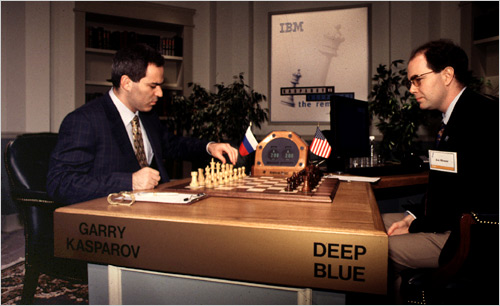
\includegraphics[width=0.8\textwidth]{figs/intro/deep_blue_1.png}

        1997年5月11日,国际象棋世界冠军卡斯帕罗夫与IBM公司的超级电脑深蓝(Deep Blue)对弈。
    \end{column}
    \begin{column}[T]{.5\linewidth}
      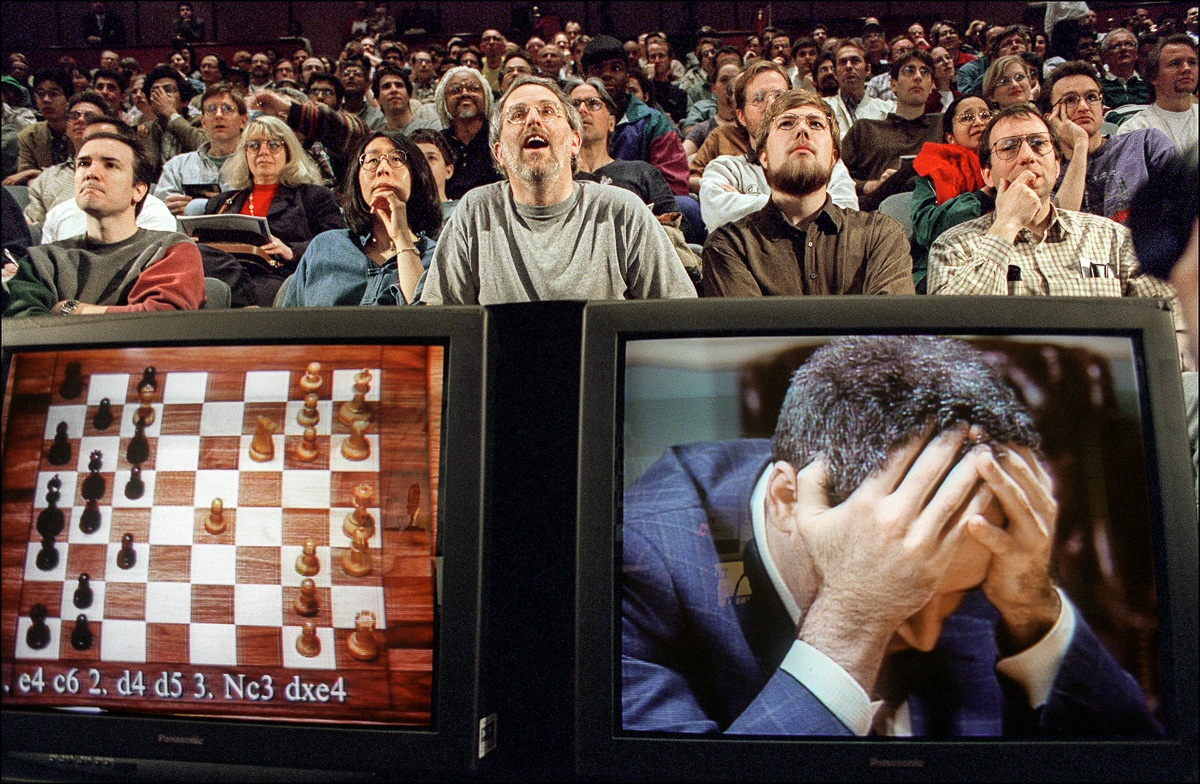
\includegraphics[width=0.8\textwidth]{figs/intro/deep_blue_2.png}

      棋迷在纽约通过电视观战。当日,卡斯帕罗夫在纽约再次负于深蓝,从而在当年的
      “人机大战”中以一胜二负三和的战绩败北。
    \end{column}
  \end{columns}
\end{frame}

\begin{frame}[fragile]
  \frametitle{~}
  \begin{columns}
    \begin{column}[T]{.65\linewidth}
      \begin{enumerate}
      \item 深蓝重量达1.4吨,有32个CPU,每个CPU有8块专门为进行国际象棋对弈设计
        的处理器,平均运算速度为每秒200万步。

        \item 总计256块处理器集成在IBM研制的RS6000/SP并行计算系统中,从而拥有每
          秒超过2亿步的惊人速度。

      \item IBM研制小组向深蓝输入了100年来所有国际特级大师开局和残局的下法。美国
        特级大师本杰明将他对象棋的理解编成程序教给深蓝。虽不会思考,但它无穷无尽
        的计算能力在很大程度上弥补了这一缺陷。
      \end{enumerate}
    \end{column}
    \begin{column}[T]{.3\linewidth}
      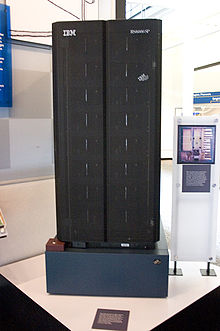
\includegraphics[width=0.8\textwidth]{figs/intro/deep_blue_3.png}
    \end{column}
  \end{columns}
\end{frame}

\begin{frame}[fragile]
  \frametitle{~}
  \begin{columns}
    \begin{column}[T]{.65\linewidth}
      \begin{enumerate}
      \item 模型: 棋盘、棋子的表示
      \item 算法: 对弈的规则和策略
        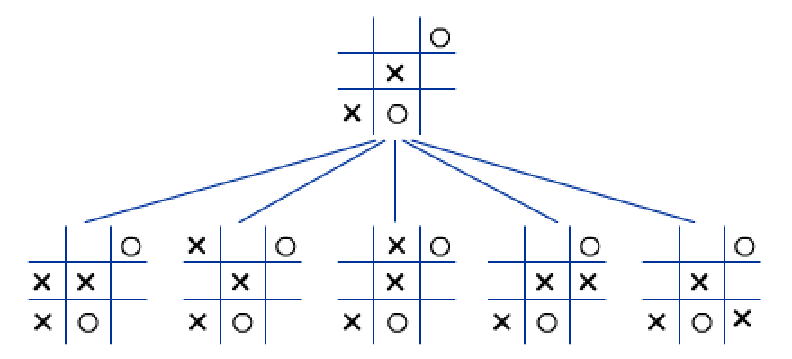
\includegraphics[width=0.8\textwidth]{figs/intro/chess_2.png}
      \item 对弈的本质即在该空间里进行有效的搜索
      \end{enumerate}
    \end{column}
    \begin{column}[T]{.3\linewidth}
      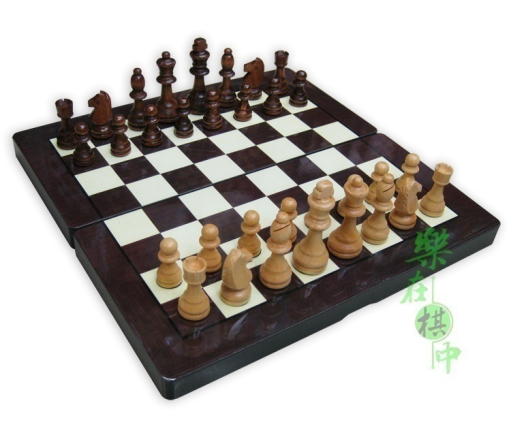
\includegraphics[width=0.8\textwidth]{figs/intro/chess_1.png}
    \end{column}
  \end{columns}
\end{frame}

\begin{frame}[fragile]
  \frametitle{~}

  \begin{columns}
    \begin{column}[T]{.5\linewidth}
      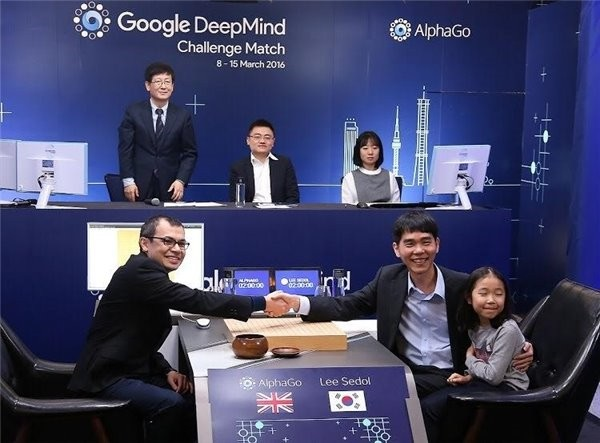
\includegraphics[width=0.8\textwidth]{figs/intro/alphago_1.png}

      2016年3月9日,Google旗下的AlphaGo电脑击败韩国九段棋手李世石。
    \end{column}
    \begin{column}[T]{.5\linewidth}
      
\includegraphics[width=0.8\textwidth]{figs/intro/alphago_2.png}

      2017年5月27日,世界排名第一的人类棋手柯洁负于AlphaGo,人机大战2.0定格在了0:3。
    \end{column}
  \end{columns}
\end{frame}

\begin{frame}[fragile]
  \frametitle{~}

  \begin{itemize}
  \item 对于擅长于计算的计算机来说,围棋的难度在很大程度上来自于19*19路棋盘背后
    所蕴含的巨大的无法穷尽的变化( 3361种下法),这是基于“穷尽法”的“深蓝”无法在
    围棋上战胜人类的原因。

  \item AlphaGo取得如此成绩,关键是深度学习和类神经网络技术。
  \item AlphaGo将棋盘看作是一个19*19像素构成的图片,利用类似于卷积神经网络的技术
    预测下一步走法。
  \end{itemize}
\end{frame}

\begin{frame}[fragile]
  \frametitle{大语言模型加速技术}
  \begin{easylist}
    & Page Attention
   & Flash Attention
  \end{easylist}

  数据结构与算法的优化,可以解决LLM落地应用的速度问题。
\end{frame}

\begin{frame}[fragile]
  \frametitle{依赖于高效的搜索}
  \begin{easylist}
    & 如何快速的搜索到右方的图例?
  \end{easylist}

    \begin{columns}
    \begin{column}[T]{.6\linewidth}
      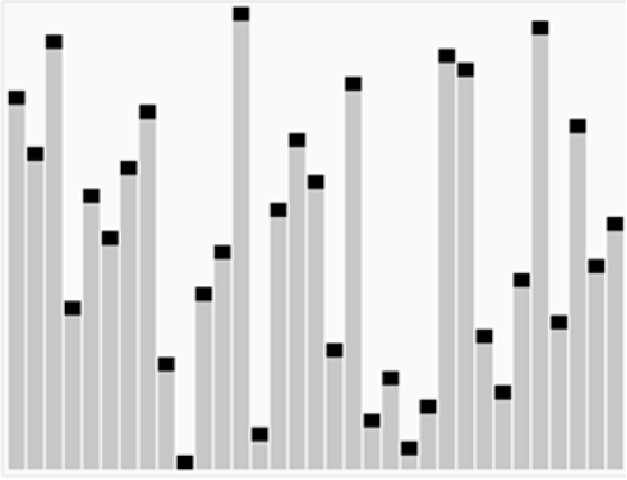
\includegraphics[width=0.8\textwidth]{figs/intro/sort_demo_1.png}
    \end{column}
    \begin{column}[T]{.5\linewidth}
      \vspace{2cm}
      
\includegraphics[width=0.2cm]{figs/intro/sort_demo_2.png}
    \end{column}
  \end{columns}

\end{frame}

\begin{frame}[fragile]
  \frametitle{依赖于高效的搜索}
  \begin{easylist}
    & 如何快速的搜索到右方的图例?
  \end{easylist}

    \begin{columns}
    \begin{column}[T]{.6\linewidth}
      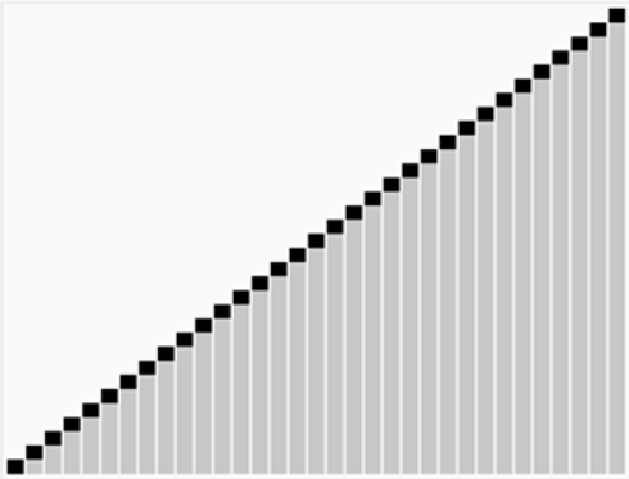
\includegraphics[width=0.8\textwidth]{figs/intro/sort_demo_3.png}
    \end{column}
    \begin{column}[T]{.5\linewidth}
      \vspace{2cm}
      
\includegraphics[width=0.2cm]{figs/intro/sort_demo_2.png}
    \end{column}
  \end{columns}

    数据有序有利于查找。需要对数据进行高效的组织/排序。
\end{frame}

\begin{frame}[fragile]
  \frametitle{Algorithms + Data Structures = Programs}

  \begin{easylist}
    & 算法
    && 处理问题的策略/操作步骤
    & 数据结构
    && 静态数据表示的数学模型(以及必须的操作)
    & 程序
    && 为计算机处理问题编制的一组指令集
  \end{easylist}

  \begin{tcolorbox}[standard jigsaw, opacityback=0, colframe=red]
    数据结构:研究描述现实世界实体的数学模型及其上的操作在计算机中的表示和实现。
  \end{tcolorbox}

\end{frame}

\begin{frame}[fragile]
  \frametitle{FAQ}
  \begin{enumerate}
  \item 数据结构是又一门编程课吗?
  \item 不会C/Java/Python语言怎么办?
  \item 用别的语言学习数据结构可以吗?
  \item 怎样学好数据结构?
  \end{enumerate}
\end{frame}


\subsection{基本概念和术语}
\begin{frame}[fragile]
  \frametitle{基本概念和术语}

  \begin{easylist}
  &  基本概念和术语
  &  抽象数据类型的表示与实现
  &  算法和算法分析
  \end{easylist}
\end{frame}

\begin{frame}[fragile]
  \frametitle{基本概念}

  \begin{easylist}
    & 1、数据 (Data)

    && 对客观事物的符号表示,在计算机科学中特指所有能被输入到计算机中并能被计算
    机程序处理的符号的总称。数据是程序加工的“原料”。

    && 例:一个文字处理程序的处理对象是字符串。

    & 2、数据元素 (Data Element)

    && 数据的基本单位,在计算机程序中通常{\color{red}作为一个整体}被考虑和处理。

    && 例:一本书,一条学生记录。

    && 数据元素可由若干数据项 (Data Item)组成。
  \end{easylist}
\end{frame}

\begin{frame}[fragile]
  \frametitle{基本概念}

  \begin{easylist}
    & 3、数据对象 (Data Object):性质相同的数据元素的集合,是数据的一个子集。

    && 例1: 整数数据对象, $N=\{0, 1, 2, \cdots \}$
    && 例2: 字符数据对象, $C=\{'A', 'B', \cdots \}$

    & 4、数据类型 (Data Type): 一个值的集合和定义在这个值集上的一组操作的总称。

    && 原子类型

    &&& 不可分解的数据类型

    &&& 如:整型、字符型、指针型、空类型…

    && 结构类型

    &&& 可分解为若干成分

    &&& 如:数组由分量组成,分量可以是整型,也可以是数组.
  \end{easylist}
\end{frame}

\begin{frame}[fragile]
  \begin{tcolorbox}[colframe=red, title=数据结构]
      数据结构 (狭义上) 是相互之间存在一种或多种特定关系的数据元素的集合。
  \end{tcolorbox}

  \begin{easylist}
    & 逻辑结构
    && 集合、线性结构、树形结构、图状或网状结构

    & 物理结构:数据结构在计算机中的表示/映像
    && 数据元素的表示是结点 (node),即在计算机内用若干位组合起来表示一个数据元素。
    && 数据关系的表示有顺序映像和非顺序映像两种,由此得到顺序存储结构和链式存储结构。
  \end{easylist}
\end{frame}

\begin{frame}[fragile]
  \frametitle{物理结构}
  \begin{easylist}
    & 顺序映像 (顺序存储结构)

    && 逻辑上相邻的数据元素存储在物理位置上相邻的存储单元中比如在高级语言中的“一
    维数组”。

    & 非顺序映像 (链式存储结构)

    && 数据元素可以存储在计算机内任意位置上,它们的逻辑关系用指针来链接。比如在
    高级语言中的“指针”。
  \end{easylist}
\end{frame}

\begin{frame}[fragile]
  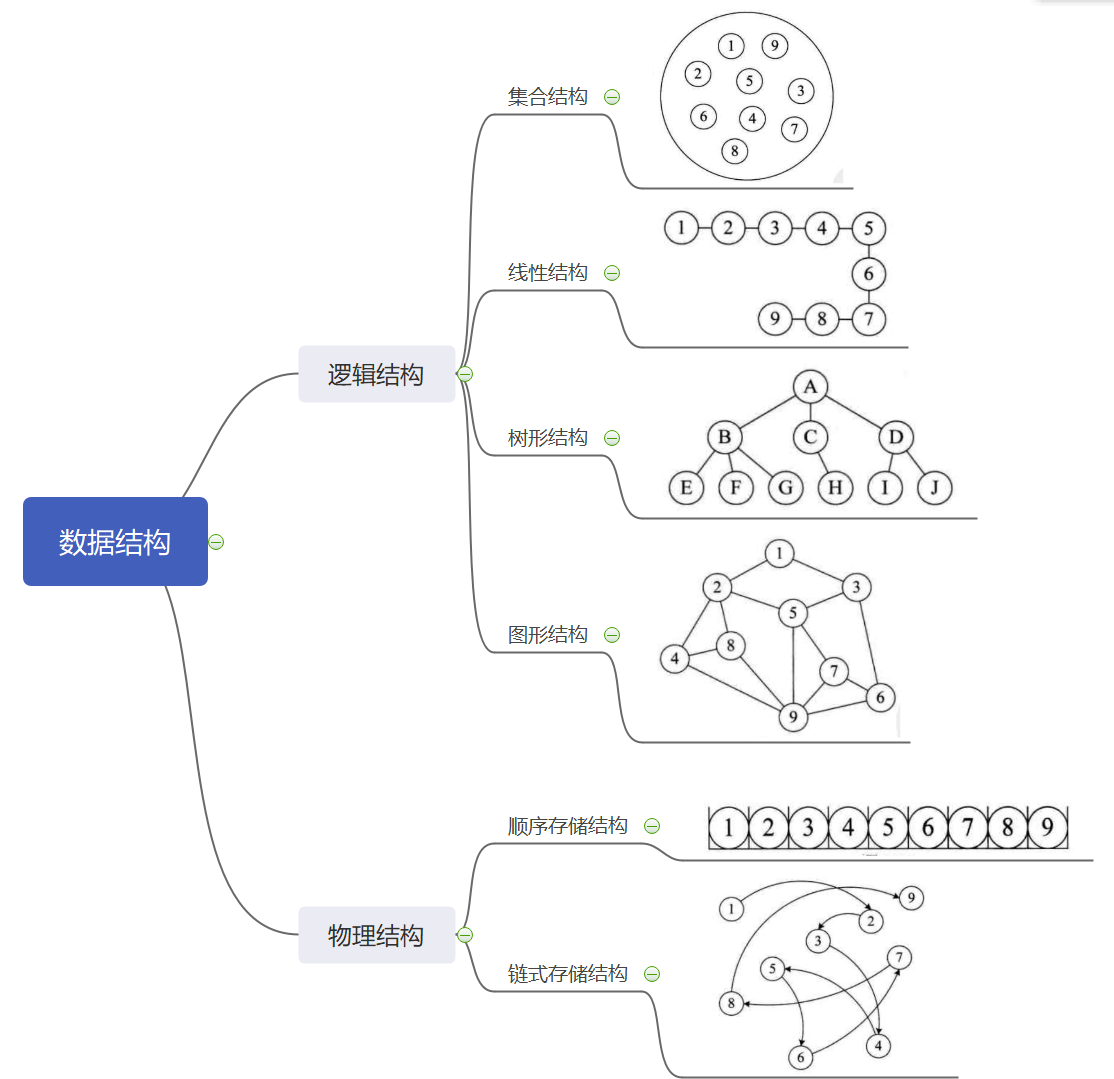
\includegraphics[width=0.7\textwidth]{figs/intro/ds_category.png}
\end{frame}


\subsection{抽象数据类型的表示和实现}
\begin{frame}[fragile]
  \frametitle{抽象数据类型的表示和实现}
  \begin{easylist}
    & 抽象数据类型 (Abstract Data Type)是指一个数学模型以及定义在该模型上的一组操作。

    && 例如,矩阵 +(求转置、加、乘、求逆、求特征值)构成一个矩阵的抽象数据类型

    &&“抽象”在于数据类型的数学抽象特性,与具体表示和实现无关。
  \end{easylist}
\end{frame}

\begin{frame}[fragile]
  \frametitle{抽象数据类型的示例}
  \scriptsize
  \begin{minted}{c}
ADT Complex {
   数据对象:D = {e1,e2 | e1,e2 in RealSet  }
   数据关系:R1 = {<e1,e2> | e1是复数的实数部分,  e2 是复数的虚数部分 }
   基本操作:
       InitComplex( &Z, v1, v2 )
          操作结果:构造复数Z,实部和虚部分别被赋以参数v1和v2的值.
      DestroyComplex( &Z)
          操作结果:复数Z被销毁.
      GetReal( Z, &realPart )
          初始条件:复数已存在。
          操作结果:用realPart返回复数Z的实部值.
     GetImag( Z, &ImagPart )
          初始条件:复数已存在。
          操作结果:用ImagPart返回复数Z的虚部值.
     Add( z1,z2, &sum )
          初始条件:z1,z2是复数。
          操作结果:用sum返回两个复数z1,z2的和值.
} ADT Complex
  \end{minted}
\end{frame}

\subsection{算法和算法分析}
\begin{frame}[fragile]
  \frametitle{算法和算法分析}
  \begin{itemize}
  \item 基本概念和术语
  \item 抽象数据类型的表示与实现
  \item 算法和算法分析
  \end{itemize}
\end{frame}

\begin{frame}[fragile]
  \frametitle{Alkhwarizmi与Algorithm}
  \begin{itemize}
  \item Alkhwarizmi(约780~约850),数学家,代数与算术的整理者。阿拉伯文
    Alkhwarizmi 原意是来自 (al-) 花剌子模 (Khwarizmi) 。
  \item Alkhwarizmi在当时的学问中心巴格达,服务于宫廷。他写了一本有关代数的书,
    这本书转成欧文,书名逐渐简化为algebra(代数)。
  \item 后来Alkhwarizmi又引进了印度数字发展算术,后经 Fibonacci(1170~1250年)
    引入欧洲。欧洲人把 Alkhwarizmi这个字拉丁化,称用十进位印度阿拉伯数字来进行有
    规则可寻的计算的算术为 Algorithm。后来算术转用其它的字(如 arithmetic), 而
    algorithm 则成为计算机科学的行话。
  \end{itemize}
\end{frame}

\begin{frame}[fragile]
  \frametitle{算 法 (Algorithm) }
  \begin{easylist}
    & 算法是对特定问题求解步骤的一种描述,是指令的有限序列,其中每一条指令表示一
    个或多个操作。算法可以看做是从输入到输出的一个映射。

    && Input $\rightarrow$ Ouput

    & 算法的描述

    && 自然语言

    && 程序流程图

    && 伪码: 它忽略高级程序设计语言中一些严格的语法规则与描述细节,因此比程序设
    计语言更容易描述和被人理解,而比自然语言更接近程序设计语言。它虽然不能直接执
    行但很容易被转换成高级语言。

    && 编程语言
  \end{easylist}
\end{frame}

\begin{frame}[fragile]
  \frametitle{试写出[9,2,5,1,6,7,10]经过下列程序处理后的序列。}

  \begin{minted}{c}
//冒泡法
void bubble (int a[], int n) {
  for (i=n-1; i>=1; i - -) {
    for (j=0; j<i; j++)
      if (a[j]>a[j+1]) {
        swap(&a[j],&a[j+1]);
      }
  }
}
  \end{minted}

  \begin{easylist}
    & $i = n - 1 $ $\cdots$

    & $i = n - 2 $ $\cdots$
  \end{easylist}
\end{frame}

\begin{frame}[fragile]
  \frametitle{算法设计的要求}
  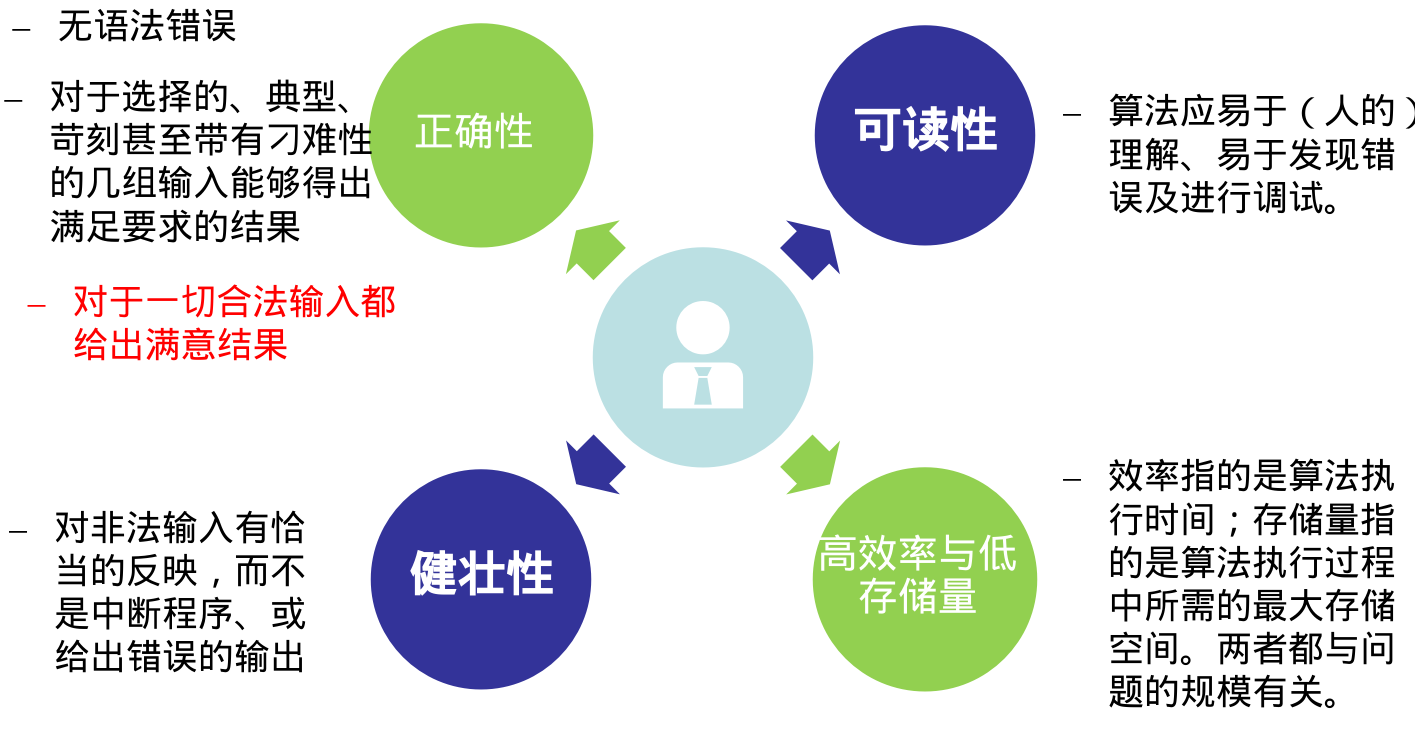
\includegraphics[width=0.9\textwidth]{figs/intro/algorithm_req.png}
\end{frame}

\begin{frame}[fragile]
  \frametitle{算法效率}
  \begin{easylist}
    & 算法执行时间需通过依据该算法编制的程序在计算机上运行时所消耗的时间来度量。

    & 相关影响因素包括:

    && 机器硬件配置直接影响计算机执行指令的速度
    && 编写程序的语言:越高级, 效率越低
    && 算法选用的策略
    && 问题的规模:规模越大, 耗时越久
    && 编译程序产生的机器代码的质量
  \end{easylist}
\end{frame}

\begin{frame}[fragile]
  \frametitle{快递员配送包裹}
  \begin{easylist}
    & 假定快递员以恒定速度行驶,比较下面的方案

    && 方案1:配送n个包裹的总时间为$n^2 + n$

    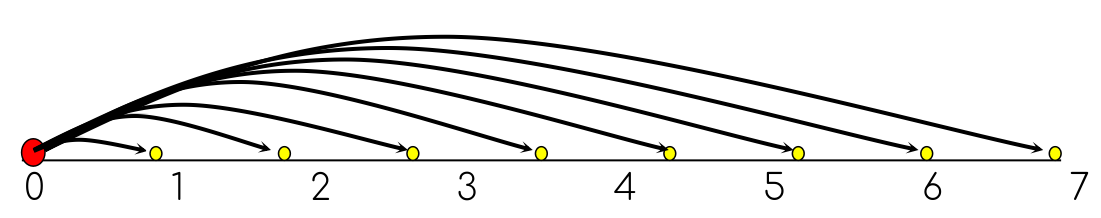
\includegraphics[width=0.8\textwidth]{figs/intro/postman1.png}

    && 方案2:配送n个包裹的总时间为2n

    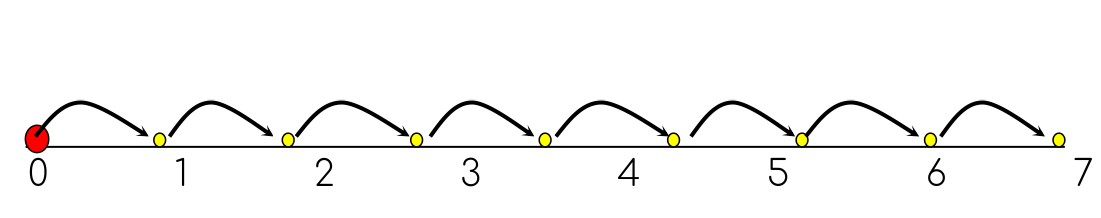
\includegraphics[width=0.8\textwidth]{figs/intro/postman2.png}
  \end{easylist}
\end{frame}

\begin{frame}[fragile]
  \frametitle{各函数的增长率}
  在问题规模增长时,算法执行时间必定也会增长。我们关心的是这个执行次数以什么样的数量级(增长率)增长。

  \begin{center}
    \begin{tabular}{| r | r | r | r | r |}
      \hline
      $n$ & $long_2{n}$ & $n \cdot log_2 n$ & $n^2$ & $2^n$ \\ \hline
      1 & 0 & 0 & 1 & 2 \\ \hline
      2 & 1 & 2 & 2 & 4 \\ \hline
      4 & 2 & 8 & 16 & 16 \\ \hline
      8 & 3 & 24 & 64 & 256 \\ \hline
      16 & 4 & 64 & 256 & 65,536  \\ \hline
      32 & 5 & 160 & 1,024 & 4,294,967,296  \\ \hline
    \end{tabular}
  \end{center}
\end{frame}

\begin{frame}[fragile]
  \frametitle{观察$g(n)$和$f(n)$的相对增长趋势}

  \begin{center}
    \begin{tabular}{| r | r | r |}
      \hline
      $n$ & $g(n)=n^2$ & $f(n)=n^2+4n+20$ \\ \hline
      10 & 300 & 360  \\ \hline
      50 & 2,500 & 2,720  \\ \hline
      100 & 10,000 & 10,420  \\ \hline
      1,000 & 1,000,000 & 1,004,020  \\ \hline
      10,000 & 100,000,000 & 100,040,020  \\ \hline
    \end{tabular}
  \end{center}

  \begin{easylist}
    & 当n变得很大时,$n^2$成为主导项,通过$g(n)$的变化情况就可以预测$f(n)$的变化。

    \[O(c_1 n^k + c_2 n^{k-1} + \cdots + c_k) = O(n^k)\]

    & 例如,$T(n)=3n^ 2+ 4n + 20$,记为$O(n^2)$
  \end{easylist}
\end{frame}

\begin{frame}[fragile]
  \frametitle{Big-O Complexity Chart}
  \begin{columns}
    \begin{column}[T]{.6\linewidth}            %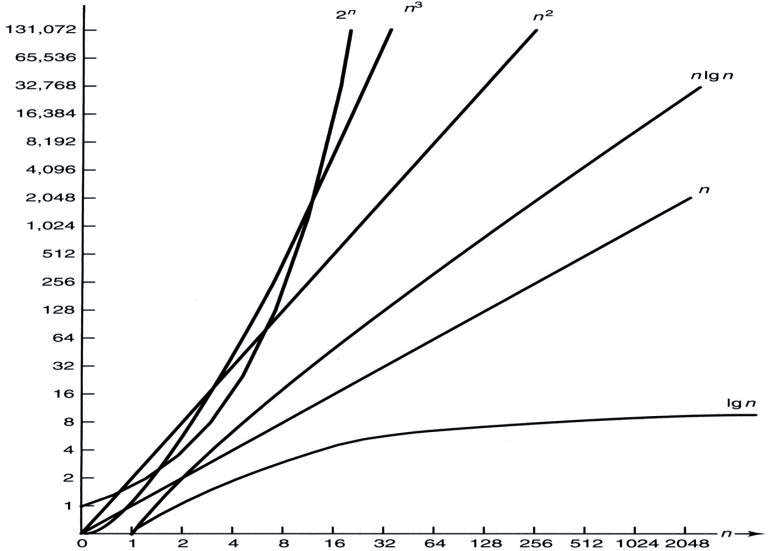
\includegraphics[width=1.0\textwidth]{figs/intro/Growth-Rates-of-Some-Common-Complexity-Functions.png}
        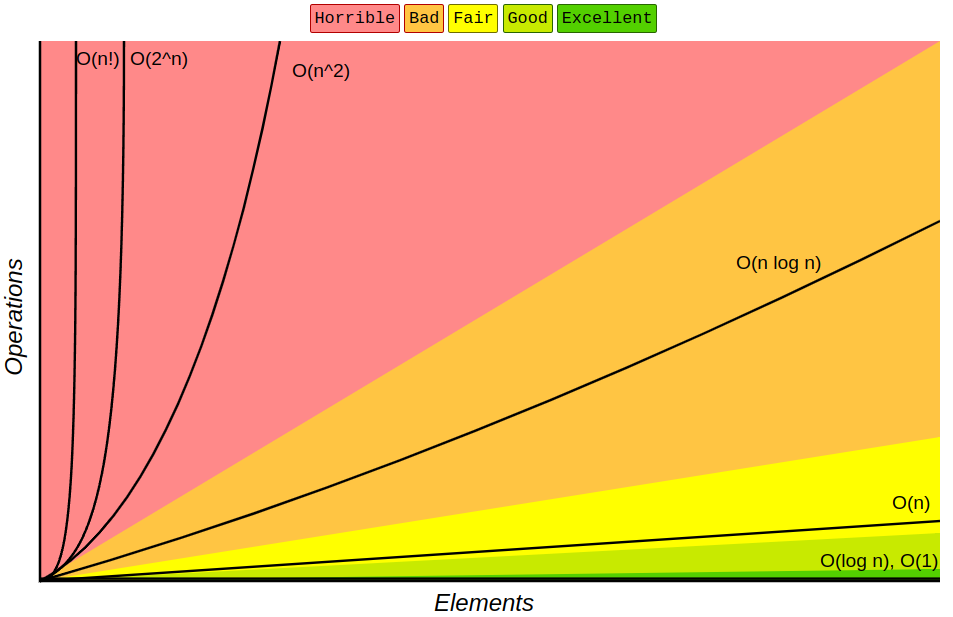
\includegraphics[width=1.0\textwidth]{figs/intro/bigocheatsheet.png}

        From: \url{https://www.bigocheatsheet.com}
    \end{column}
    \begin{column}[T]{.4\linewidth}
      \scriptsize
      From better to worse:

      \begin{tabular}{l l}
        \hline
        $O(1)$ & constant time \\ \hline
        $O(\log n)$ & log time \\ \hline
        $O(n)$ & linear time \\ \hline
        $O(n \log n)$ & log linear time \\ \hline
        $O(n^2)$ & quadratic time \\ \hline
        $O(n^3)$ & cubic time \\ \hline
        $O(2^n)$ & exponential time \\ \hline
      \end{tabular}
    \end{column}
  \end{columns}
\end{frame}

\begin{frame}[fragile]
  \frametitle{大O表示法}
  \begin{easylist}
    & 算法的(渐近)时间复杂度记作: $T(n) = O(f(n))$

    && 表示随问题规模$n$的增大,算法执行时间的增长率和$f(n)$的增长率相同。

    & 通常是从算法中选取一种最基本的元操作,以该操作重复执行的次数(频度)来度量算法效率
  \end{easylist}
\end{frame}

\begin{frame}[fragile]
  \frametitle{例:矩阵相乘 (C代码示例)}
  \begin{minted}{c}
    for (i=1; i<=n; i++)
      for (j=1; j<=n; j++) {
        c[i][j] = 0;
        for (k=1; k<=n; k++)
          c[i][j] =c[i][j]+ a[i][k] * b[k][j]; // 该语句可看作元操作
      }
  \end{minted}

  \begin{tcolorbox}
    整个算法的执行时间与元操作重复执行的次数$n^3$成正比,记作$T(n) = O(n^3)$
  \end{tcolorbox}
\end{frame}

\begin{frame}[fragile]
  \frametitle{例:矩阵相乘 (Python代码示例)}
  \begin{minted}{python}
n = 3
a = [[1,2,3],[4,5,6], [7,8,9]]
b = [[1,2,3],[4,5,6], [7,8,9]]

c = [ [0]*n for _ in range(n) ]
for i in range(n):
    for j in range(n):
        c[i][j] = 0
        for k in range(n):
            c[i][j] = c[i][j] + a[i][k] * b[k][j]
  \end{minted}

  \begin{tcolorbox}
    整个算法的执行时间与元操作重复执行的次数$n^3$成正比,记作$T(n) = O(n^3)$
  \end{tcolorbox}
\end{frame}

\begin{frame}[fragile]
  \frametitle{请观察 [10,9,7,6] 和 [6,7,9,10]在处理上的不同。}
  \begin{minted}{c}
    void bubble(int a[], int n) {
      for (i=n-1; i>=1; i - -) {
        for (j=0; j<i; j++)
          if (a[j]>a[j+1]) {
              swap(&a[j],&a[j+1]);
          }
      }
    }
  \end{minted}

  \pause

  \begin{itemize}
  \item 若初始文件是正序的,一趟扫描即可完成排序。
  \item 若初始文件是反序的,需要进行$n-1$趟排序。
  \item \color{red}计算平均复杂度,或最坏情况下的时间复杂度.
  \end{itemize}
\end{frame}

\begin{frame}[fragile]
  \frametitle{~}
  \begin{itemize}
    \item 最好情况的时间复杂度 (初始文件是正序的)

      [6,7,9,10] --- 一趟扫描即可完成排序,共计$n-1$次比较(0次交换)。

      冒泡排序最好情况的时间复杂度为$O(n)$

   \item 最坏情况的时间复杂度 (初始文件是反序的)

     [10,9,7,6] --- 需要进行n-1趟扫描,每趟进行$i$次比较+交换$(1\leq i \leq n-1)$ ,共计$\dfrac{n (n-1)}{2}$次比较+交换。

     冒泡排序的最坏情况的时间复杂度为$O(n^2)$

  \end{itemize}
\end{frame}

\begin{frame}[fragile]
  \frametitle{算法的存储空间需求 (内存)}
  \begin{easylist}
    & 算法需要为: 输入数据、程序、辅助变量提供存储空间。
    & 算法的空间复杂度: $S(n) = O(g(n))$
    & 随着问题规模增大,算法运行所需存储量的增长率与$g(n)$的增长率相同。
    & 若所需存储量依赖于特定的输入,则通常按最坏情况考虑。
    & 相对于时间复杂度而言,空间复杂度在很多时候不需进行分析。
  \end{easylist}
\end{frame}

\begin{frame}[fragile]
  \frametitle{小结}

  \begin{enumerate}
  \item 数据结构 研究非数值计算的程序设计问题中计算机的操作对象以及它们之间的关系和操作。
  \item 数据、数据元素、数据对象、数据结构的概念
  \item 常见的基本数据结构
  \item 以大O表示法分析算法时间复杂度
  \end{enumerate}
\end{frame}
